\chapter*{Dodatek}
\addcontentsline{toc}{chapter}{Dodatek}
\markboth{DODATEK}{}
\label{dodatek}

\section{Instalace pluginu}

Popis instalace pluginu je uveden pro software QGIS nastavený v anglickém jazyce. 

\subsection{Instalace pluginu skrz QGIS repozitář}

Pro nainstalování pluginu \textit{GTFS Loader} v softwaru QGIS se nejprve přes menu vybere 
panel \textit{Plugins} a poté z nabídky panelu se vybere možnost \textit{Manage and Install Plugins...}.
Poté se otevře dialogové okno pro výběr instalace pluginu z QGIS repozitáře, zadá se název
plugin a stiskne se tlačítko \textit{Install Plugin} 

\begin{figure}[H] \centering
    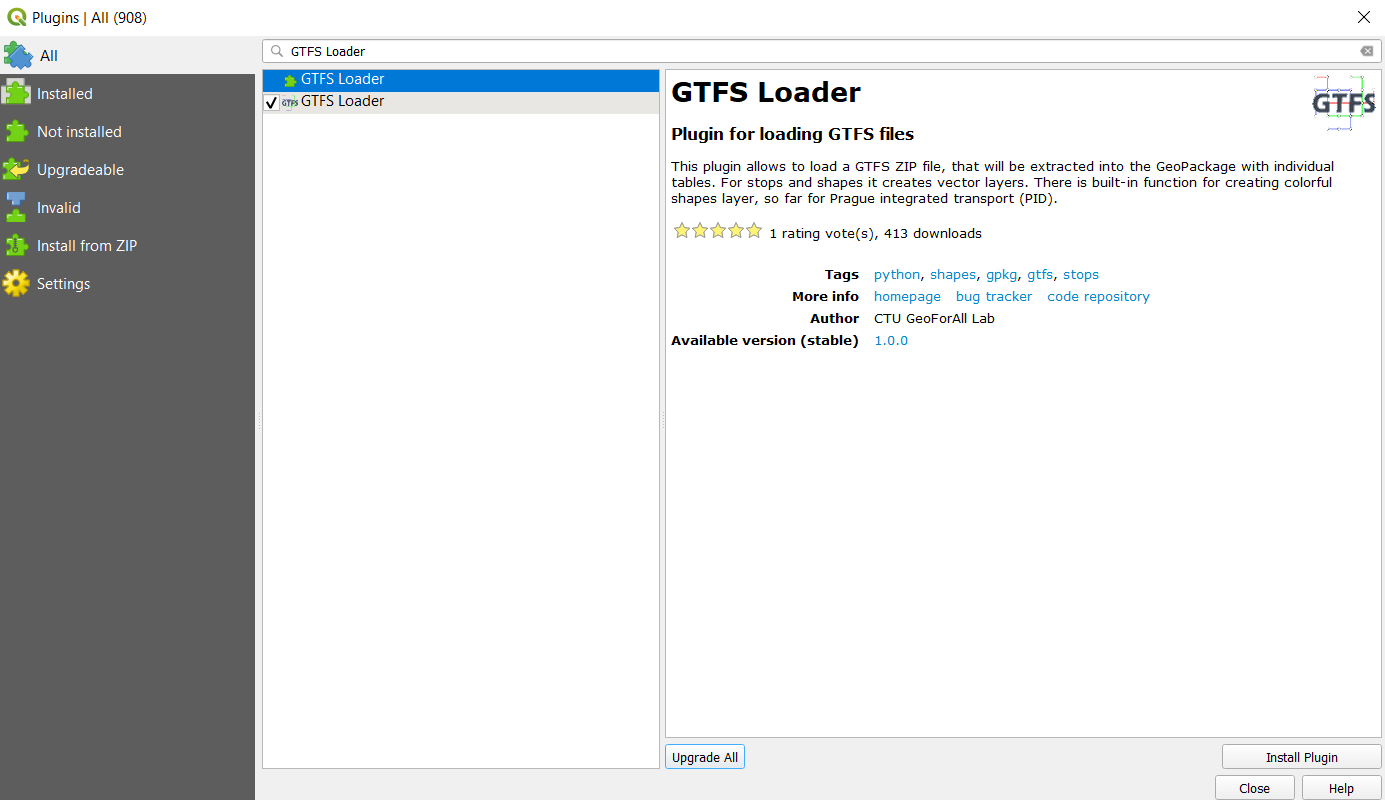
\includegraphics[width=400pt]{./pictures-dodatek/repositary.png}
    \caption[Dialogové okno pro výběr instalace pluginu z QGIS repozitáře]{Dialogové okno pro výběr instalace pluginu z QGIS repozitáře}
	\label{fig:repositary}              
\end{figure} 

\subsection{Instalace pluginu skrz ZIP soubor}

\href{https://github.com/ctu-geoforall-lab/qgis-gtfs-plugin/tree/pid\_zones}
{https://github.com/ctu-geoforall-lab/qgis-gtfs-plugin/tree/pid\_zones}

\begin{figure}[H] \centering
    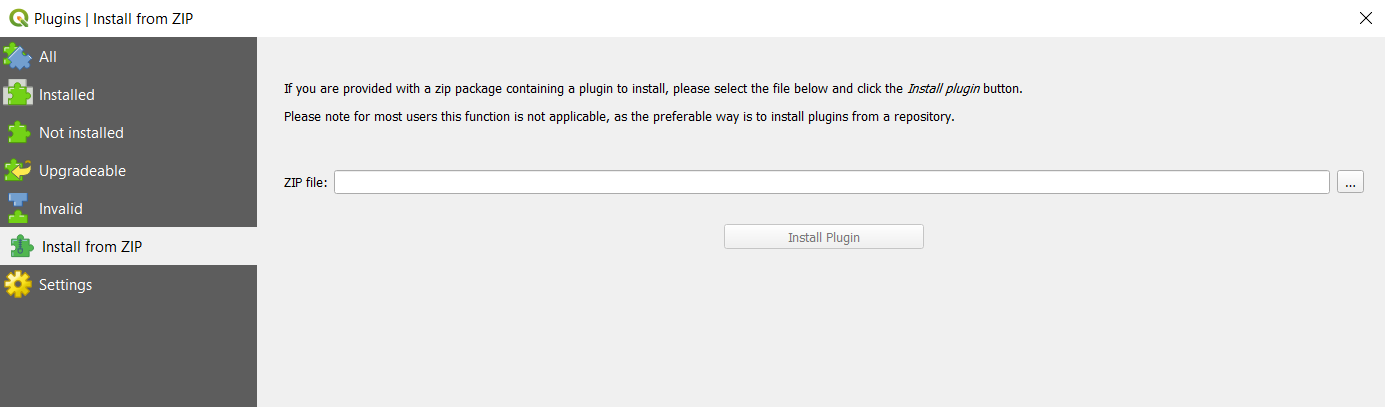
\includegraphics[width=400pt]{./pictures-dodatek/zip.png}
    \caption[Dialogové okno pro výběr ZIP souboru]{Dialogové okno pro výběr ZIP souboru}
	\label{fig:zip}              
\end{figure} 

